\documentclass[11pt]{article}

\usepackage[]{ACL2023}

\usepackage{times}
\usepackage{latexsym}

\usepackage[T1]{fontenc}

\usepackage[utf8]{inputenc}

\usepackage{microtype}

\usepackage{inconsolata}

\usepackage{graphicx}

\title{Asking Clarifying Questions for Conversational Search}

\author{
  Ansh Bisht \and
  Jordan Dickson \and
  Jack Harrison \and
  Ruben Lazell \and
  Andrew Taison  \\
  School of Computing, Engineering and the Built Environment, \\
  Edinburgh Napier University \\
  Matric Numbers: 40527530, 40545300, 40537035, 40679914, 40538519
}


\begin{document}
\maketitle
\begin{abstract}
Short abstract.
\end{abstract}


\section{Introduction}
Brief context of problem - why clarifying Q's matter.
What is the goal.
Structure of the paper.

\section{Related Work}
Existing systems, prior research etc.

\section{Methodology}



\subsection{System Overview}
The system for the clarification model was constructed through a series of key components:User queries with a question for the system, RASA for application control of the entire system, Best Matching 25 (BM25) model for matching the queries on the Wikipedia Dataset, and SBERT for constructing Sentence Similarity Scores to rank the best results. The dependencies and relationships of these components are illustrated below.

\begin{figure}[htbp]
  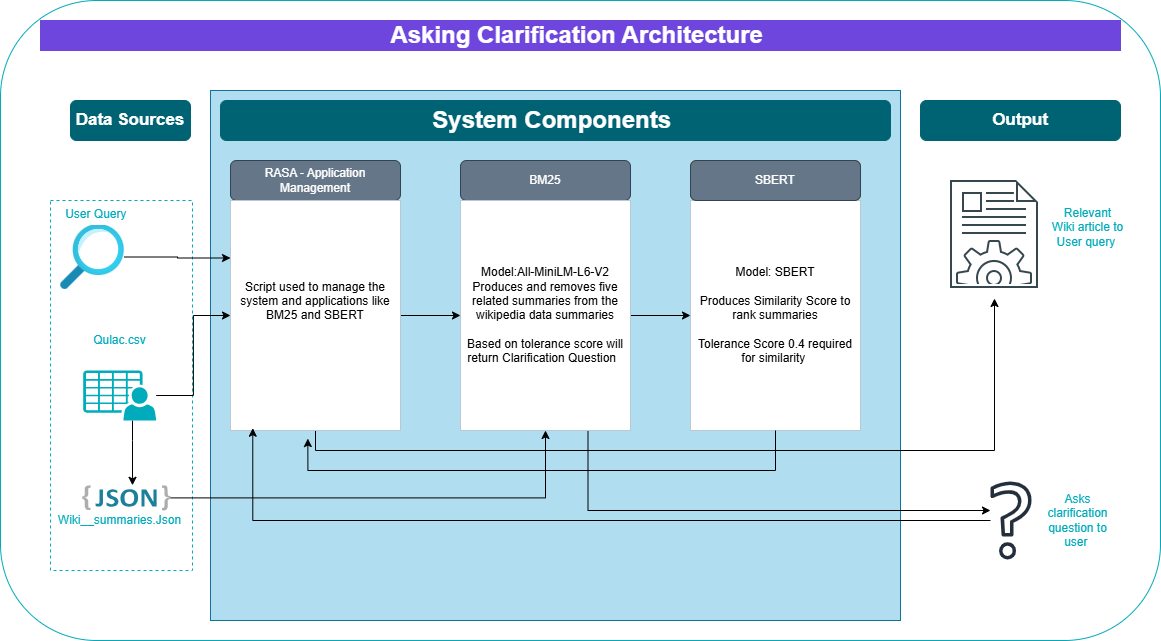
\includegraphics[width=\linewidth]{./img/system_diagram.png}
  \caption{Enter Caption}
  \label{fig:sys_diag}
\end{figure}

\subsection{Qulac Dataset}
The Qulac data was one of the primary datasets for this system. One of the initial steps was to appropriately shape the data to work with the other elements within our system. The transformations for cleaning this dataset were performed initially in Python using the Pandas library, and the resulting CSV was stored within a Google Drive directory.

\subsection{Original Qulac Dataset}
A dictionary with query keys and a list of relevant facet descriptions (user intents).

\subsection{Clean Qulac Schema}
\renewcommand{\arraystretch}{1.2} % increase row height for readability

\begin{table}[ht]
  \centering
  \caption{Dataset Column Descriptions}
  \label{tab:dataset-columns}
  \begin{tabular}{@{} l l p{5cm} @{}}
    \hline
    \textbf{Column Name}  & \textbf{Type}    & \textbf{Description}                        \\ 
    \hline
    Index                 & String           & Facet index based on word string.            \\ 
    Category Name         & String           & Name of the broader category of the dataset. \\ 
    Facet Description     & String           & Detailed description of the facet.           \\ 
    Col 1                 & String           & Response 1.                                  \\ 
    Col 2                 & String           & Response 2.                                  \\ 
    Col 3                 & String           & Response 3.                                  \\ 
    Col 4                 & String           & Response 4.                                  \\ 
    New Index             & Integer          & Row index counter.                           \\ 
    \hline
  \end{tabular}
\end{table}

One of the most important features of our Qulac Dataset was the facet descriptions, as they were used to derive the Wikipedia Summaries.

\subsection{Wikipedia Summaries}
The Wikipedia summaries were generated using a series of GET responses contained within a Python script on the Wikipedia API. The aim was to generate five summaries per index \textendash{} topic of the facet \textendash{} relating to the user's query.

\begin{figure}[htbp]
  \centering
  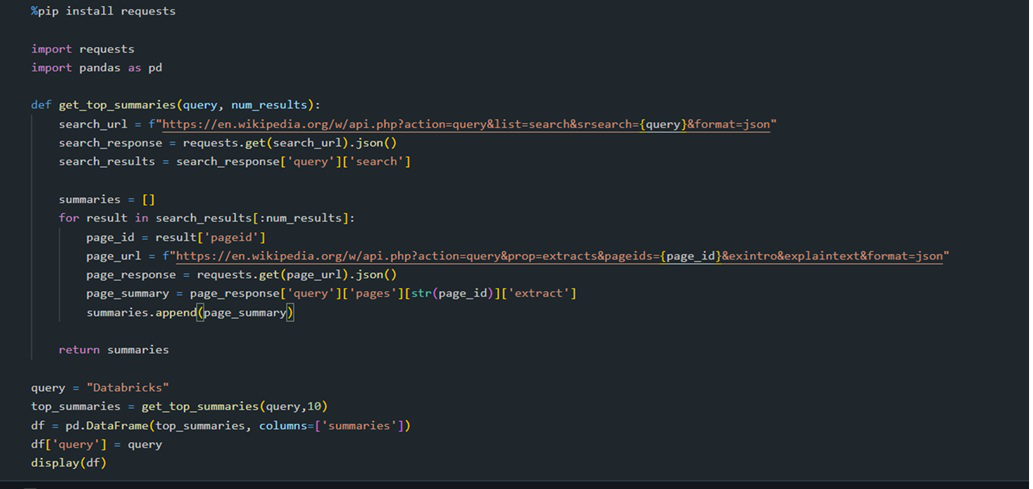
\includegraphics[width=\linewidth]{./img/wiki.png}
  \caption{Wikipedia Summaries Generation}
  \label{fig:wikipedia method}
\end{figure}


Once completed, the Wikipedia Summaries were shaped into the cleaned dataset above. These summaries were required for BM25 later in the project. In a larger project, the Wikipedia API could be used to return the entire articles, but this would come at a cost of time, compute, and complexity.


\subsection{{RASA}}
RASA is the machine learning framework used for building this system. It is used to manage the dialogue by deploying the suitable models. For this project, RASA deploys BM25 and SBERT, allowing the system to function cohesively.

\subsection{Best Matching 25 (BM25)}
BM25 was the key AI model in matching user queries to the relevant Wikipedia summaries within the system. The model used was from Huggingface and constructed via a Python script. 
 \newline
 \newline
The documents used were the Wikipedia Summaries from the generated CSV. The result was that the system determined the need for clarification based on a tolerance score of 0.40 for similarity. A ranking was also performed using all-MiniLM-L6-v2 from HuggingFace to select the best matching summary.


\subsection{SBERT}
The final step was determining the suitability of the top-ranked result. A specialized version of BERT called SBERT from Huggingface was utilized.

Our SBERT model was fine-tuned on \texttt{sbert\_training\_data.csv}, which contained two features: context and question. Each context is a formatted string combining the initial query (tagged with \texttt{[Q]}) and the next element (a question and its answer tagged with \texttt{[A]}).

The model applied a similarity score with a tolerance threshold of 0.4. If the context and question's similarity score was above 0.4, the result was deemed suitable; otherwise, it was not ranked.


\cite{Aliannejadi2019}

\section{Evaluation}
How did we check the system works.
Describe testing process.

\section{Results and Discussion}
Sample outputs.
Summary of system behaviour.
What worked well, what didn't?
Possible improvements.

\section{Conclusion}
start here.

\section*{Limitations}
Required by ACL format, and should be AFTER conclusion.
Discuss honest limitations of the work.

\section*{Ethics Statement}
Required by ACL format. Could just be a sentence or two.
Explicit ethics statement on the broader impact of the work, or other ethical considerations.

\bibliographystyle{acl_natbib}
\bibliography{references}

\appendix

\section{Appendix}
Possibly not needed.

\end{document}
